\documentclass[manuscript, review, anonymous, screen]{acmart}


\IfFileExists{upquote.sty}{\usepackage{upquote}}{}
\IfFileExists{microtype.sty}{% use microtype if available
  \usepackage[]{microtype}
  \UseMicrotypeSet[protrusion]{basicmath} % disable protrusion for tt fonts
}{}
\makeatletter
\@ifundefined{KOMAClassName}{% if non-KOMA class
  \IfFileExists{parskip.sty}{%
    \usepackage{parskip}
  }{% else
    \setlength{\parindent}{0pt}
    \setlength{\parskip}{6pt plus 2pt minus 1pt}}
}{% if KOMA class
  \KOMAoptions{parskip=half}}
\makeatother

%%
%% This is file `sample-manuscript.tex',
%% generated with the docstrip utility.
%%
%% The original source files were:
%%
%% samples.dtx  (with options: `manuscript')
%% 
%% IMPORTANT NOTICE:
%% 
%% For the copyright see the source file.
%% 
%% Any modified versions of this file must be renamed
%% with new filenames distinct from sample-manuscript.tex.
%% 
%% For distribution of the original source see the terms
%% for copying and modification in the file samples.dtx.
%% 
%% This generated file may be distributed as long as the
%% original source files, as listed above, are part of the
%% same distribution. (The sources need not necessarily be
%% in the same archive or directory.)
%%
%%
%% Commands for TeXCount
%TC:macro \cite [option:text,text]
%TC:macro \citep [option:text,text]
%TC:macro \citet [option:text,text]
%TC:envir table 0 1
%TC:envir table* 0 1
%TC:envir tabular [ignore] word
%TC:envir displaymath 0 word
%TC:envir math 0 word
%TC:envir comment 0 0
%%
%%
%% The first command in your LaTeX source must be the \documentclass command.


% Options for packages loaded elsewhere
\PassOptionsToPackage{unicode}{hyperref}
\PassOptionsToPackage{hyphens}{url}
\PassOptionsToPackage{dvipsnames,svgnames,x11names}{xcolor}

\IfFileExists{bookmark.sty}{\usepackage{bookmark}}{\usepackage{hyperref}}

%% PANDOC PREAMBLE BEGINS


\providecommand{\tightlist}{%
  \setlength{\itemsep}{0pt}\setlength{\parskip}{0pt}}\usepackage{longtable,booktabs,array}
\usepackage{calc} % for calculating minipage widths
% Correct order of tables after \paragraph or \subparagraph
\usepackage{etoolbox}
\makeatletter
\patchcmd\longtable{\par}{\if@noskipsec\mbox{}\fi\par}{}{}
\makeatother
% Allow footnotes in longtable head/foot
\IfFileExists{footnotehyper.sty}{\usepackage{footnotehyper}}{\usepackage{footnote}}
\makesavenoteenv{longtable}
\usepackage{graphicx}
\makeatletter
\def\maxwidth{\ifdim\Gin@nat@width>\linewidth\linewidth\else\Gin@nat@width\fi}
\def\maxheight{\ifdim\Gin@nat@height>\textheight\textheight\else\Gin@nat@height\fi}
\makeatother
% Scale images if necessary, so that they will not overflow the page
% margins by default, and it is still possible to overwrite the defaults
% using explicit options in \includegraphics[width, height, ...]{}
\setkeys{Gin}{width=\maxwidth,height=\maxheight,keepaspectratio}
% Set default figure placement to htbp
\makeatletter
\def\fps@figure{htbp}
\makeatother

\usepackage{booktabs}
\usepackage{longtable}
\usepackage{array}
\usepackage{multirow}
\usepackage{wrapfig}
\usepackage{float}
\usepackage{colortbl}
\usepackage{pdflscape}
\usepackage{tabu}
\usepackage{threeparttable}
\usepackage{threeparttablex}
\usepackage[normalem]{ulem}
\usepackage{makecell}
\usepackage{xcolor}
\definecolor{mypink}{RGB}{219, 48, 122}
\makeatletter
\makeatother
\makeatletter
\makeatother
\makeatletter
\@ifpackageloaded{caption}{}{\usepackage{caption}}
\AtBeginDocument{%
\ifdefined\contentsname
  \renewcommand*\contentsname{Table of contents}
\else
  \newcommand\contentsname{Table of contents}
\fi
\ifdefined\listfigurename
  \renewcommand*\listfigurename{List of Figures}
\else
  \newcommand\listfigurename{List of Figures}
\fi
\ifdefined\listtablename
  \renewcommand*\listtablename{List of Tables}
\else
  \newcommand\listtablename{List of Tables}
\fi
\ifdefined\figurename
  \renewcommand*\figurename{Figure}
\else
  \newcommand\figurename{Figure}
\fi
\ifdefined\tablename
  \renewcommand*\tablename{Table}
\else
  \newcommand\tablename{Table}
\fi
}
\@ifpackageloaded{float}{}{\usepackage{float}}
\floatstyle{ruled}
\@ifundefined{c@chapter}{\newfloat{codelisting}{h}{lop}}{\newfloat{codelisting}{h}{lop}[chapter]}
\floatname{codelisting}{Listing}
\newcommand*\listoflistings{\listof{codelisting}{List of Listings}}
\makeatother
\makeatletter
\@ifpackageloaded{caption}{}{\usepackage{caption}}
\@ifpackageloaded{subcaption}{}{\usepackage{subcaption}}
\makeatother
\makeatletter
\@ifpackageloaded{tcolorbox}{}{\usepackage[skins,breakable]{tcolorbox}}
\makeatother
\makeatletter
\@ifundefined{shadecolor}{\definecolor{shadecolor}{rgb}{.97, .97, .97}}
\makeatother
\makeatletter
\makeatother
\makeatletter
\makeatother
%% PANDOC PREAMBLE ENDS

\setlength{\parindent}{10pt}
\setlength{\parskip}{0pt}

\hypersetup{
  pdftitle={Novel Effects of Size and Contrast Adjustments in Scatterplots},
  pdfauthor={Gabriel Strain; Andrew J. Stewart; Paul Warren; Caroline Jay},
  colorlinks=true,
  linkcolor={blue},
  filecolor={Maroon},
  citecolor={Blue},
  urlcolor={red},
  pdfcreator={LaTeX via pandoc, via quarto}}

%% \BibTeX command to typeset BibTeX logo in the docs
\AtBeginDocument{%
  \providecommand\BibTeX{{%
    Bib\TeX}}}

%% Rights management information.  This information is sent to you
%% when you complete the rights form.  These commands have SAMPLE
%% values in them; it is your responsibility as an author to replace
%% the commands and values with those provided to you when you
%% complete the rights form.
\setcopyright{acmcopyright}
\copyrightyear{2018}
\acmYear{2018}
\acmDOI{XXXXXXX.XXXXXXX}

%% These commands are for a PROCEEDINGS abstract or paper.
\acmConference[CHI]{Make sure to enter the correct conference title from
your rights confirmation emai}{June 03--05, 2018}{Woodstock, NY}
\acmPrice{15.00}
\acmISBN{978-1-4503-XXXX-X/18/06}

%% Submission ID.
%% Use this when submitting an article to a sponsored event. You'll
%% receive a unique submission ID from the organizers
%% of the event, and this ID should be used as the parameter to this command.
%%\acmSubmissionID{123-A56-BU3}

%%
%% For managing citations, it is recommended to use bibliography
%% files in BibTeX format.
%%
%% You can then either use BibTeX with the ACM-Reference-Format style,
%% or BibLaTeX with the acmnumeric or acmauthoryear sytles, that include
%% support for advanced citation of software artefact from the
%% biblatex-software package, also separately available on CTAN.
%%
%% Look at the sample-*-biblatex.tex files for templates showcasing
%% the biblatex styles.
%%

%%
%% The majority of ACM publications use numbered citations and
%% references.  The command \citestyle{authoryear} switches to the
%% "author year" style.
%%
%% If you are preparing content for an event
%% sponsored by ACM SIGGRAPH, you must use the "author year" style of
%% citations and references.
%% Uncommenting
%% the next command will enable that style.
%%\citestyle{acmauthoryear}


%% end of the preamble, start of the body of the document source.
\begin{document}


%%
%% The "title" command has an optional parameter,
%% allowing the author to define a "short title" to be used in page headers.
\title[Size, Contrast, and Scatterplots]{Novel Effects of Size and
Contrast Adjustments in Scatterplots}

%%
%% The "author" command and its associated commands are used to define
%% the authors and their affiliations.
%% Of note is the shared affiliation of the first two authors, and the
%% "authornote" and "authornotemark" commands
%% used to denote shared contribution to the research.


  \author{Gabriel Strain}
  \orcid{0000-0002-4769-9221}
            \affiliation{%
                  \institution{Department of Computer Science, Faculty
of Science and Engineering, University of Manchester}
                          \streetaddress{Oxford Road}
                          \city{Manchester}
                                  \country{United Kingdom}
                          \postcode{M13 9PL}
              }
        \author{Andrew J. Stewart}
  
            \affiliation{%
                  \institution{Department of Computer Science, Faculty
of Science and Engineering, University of Manchester}
                          \streetaddress{Oxford Road}
                          \city{Manchester}
                                  \country{United Kingdom}
                          \postcode{M13 9PL}
              }
        \author{Paul Warren}
  
            \affiliation{%
                  \institution{Division of Psychology, Communication and
Human Neuroscience, School of Health Sciences, Faculty of Biology,
Medicine, and Health, University of Manchester}
                          \streetaddress{Oxford Road}
                          \city{Manchester}
                                  \country{United Kingdom}
                          \postcode{M13 9PL}
              }
        \author{Caroline Jay}
  
            \affiliation{%
                  \institution{Department of Computer Science, Faculty
of Science and Engineering, University of Manchester}
                          \streetaddress{Oxford Road}
                          \city{Manchester}
                                  \country{United Kingdom}
                          \postcode{M13 9PL}
              }
      
\renewcommand{\shortauthors}{Strain et al.}

%% By default, the full list of authors will be used in the page
%% headers. Often, this list is too long, and will overlap
%% other information printed in the page headers. This command allows
%% the author to define a more concise list
%% of authors' names for this purpose.
%\renewcommand{\shortauthors}{Trovato et al.}
%%  
%% The abstract is a short summary of the work to be presented in the
%% article.
\begin{abstract}
Changing the size and contrast of points on scatterplots can be used to
systematically improve viewers' perceptions of correlation. Evidence
points to these effects being similar with regards to the mechanics
behind them, so one would expect that their combination would produce a
simple additive effect on correlation estimation. We present a fully
reproducible study in which we combine techniques for influencing
correlation perception to show that in reality, effects of changing
point size and contrast interact in a non-additive fashion. We show that
there are few limits to the extent to which we can use visual features
to change viewers' perceptions of data visualizations, and use our
results to further explain the perceptual mechanisms at play when
changing point size and contrast in scatterplots.    
\end{abstract}

%%
%% The code below is generated by the tool at http://dl.acm.org/ccs.cfm.
%% Please copy and paste the code instead of the example below.
%%
\begin{CCSXML}
<ccs2012>
 <concept>
  <concept_id>10010520.10010553.10010562</concept_id>
  <concept_desc>Computer systems organization~Embedded systems</concept_desc>
  <concept_significance>500</concept_significance>
 </concept>
 <concept>
  <concept_id>10010520.10010575.10010755</concept_id>
  <concept_desc>Computer systems organization~Redundancy</concept_desc>
  <concept_significance>300</concept_significance>
 </concept>
 <concept>
  <concept_id>10010520.10010553.10010554</concept_id>
  <concept_desc>Computer systems organization~Robotics</concept_desc>
  <concept_significance>100</concept_significance>
 </concept>
 <concept>
  <concept_id>10003033.10003083.10003095</concept_id>
  <concept_desc>Networks~Network reliability</concept_desc>
  <concept_significance>100</concept_significance>
 </concept>
</ccs2012>
\end{CCSXML}

\ccsdesc[500]{Computer systems organization~Embedded systems}
\ccsdesc[300]{Computer systems organization~Redundancy}
\ccsdesc{Computer systems organization~Robotics}
\ccsdesc[100]{Networks~Network reliability}

%%
%% Keywords. The author(s) should pick words that accurately describe
%% the work being presented. Separate the keywords with commas.
\keywords{correlation, scatterplot, perception, crowdsourced}


%%
%% This command processes the author and affiliation and title
%% information and builds the first part of the formatted document.
\maketitle

\setlength{\parskip}{-0.1pt}

\hypertarget{introduction}{%
\section{Introduction}\label{introduction}}

Scatterplots are common bivariate representations of data. They have
been extensively studied and are used for a variety of communicative
tasks. They are most commonly used to represent linear correlation, or
the degree of linear relatedness between two variables, but are also
used to represent different groups (clustering), to aid in the detection
of outliers, to characterize distributions, and to visualize non-linear
correlations. Figure~\ref{fig-tasks} contains examples of scatterplots
optimised for different tasks. There is evidence that people generally
interpret them in similar ways \citep{kay_2015}, and that they support
the interpretation of correlation significantly better than other data
visualizations \citep{li_2010}. Rapid interpretation by viewers
\citep{rensink_2014} along with low levels of interindividual variance
render scatterplots particularly suited for experimental work; they
provide important insights into perception and visualization design
while being simple to study.

While our interpretations of scatterplots are generally similar, the
accuracy of those interpretations is generally low. Viewers
systematically underestimate the correlation displayed in positively
correlated scatterplots. This holds true for direct estimation tasks
\citep{strahan_1978, bobko_1979, cleveland_1982, lane_1985, lauer_1989, collyer_1990, meyer_1992},
and estimation via bisection tasks \citep{rensink_2017}, and is
particularly pronounced between 0.2 \textless{} \emph{r} \textless{}
0.6. The COVID-19 pandemic demonstrated that even outside of
professional/office environments, lay populations are now expected to be
able to use and accurately interpret data visualizations on a daily
basis \citep{bbc_2022}. This expectation confers a responsibility on the
part of data visualization designers to design in such a way that people
with little statistical or graph training can be expected to correctly
interpret data visualizations. Doing this requires us to understand
human perception and perceptual phenomena, apply this understanding to
data visualization design, and test those designs in rigorous empirical
work. We therefore present a fully-reproducible, crowdsourced online
experiment in which we systematically alter visual features in
scatterplots to correct for a historic bias. We combine two techniques
for correcting for correlation underestimation in scatterplots and show
that the combined effect is stronger than one would expect were they
linearly additive. Through this work we also present a framework for
visualization design informed from the ground up by human perception.

\begin{figure}

{\centering 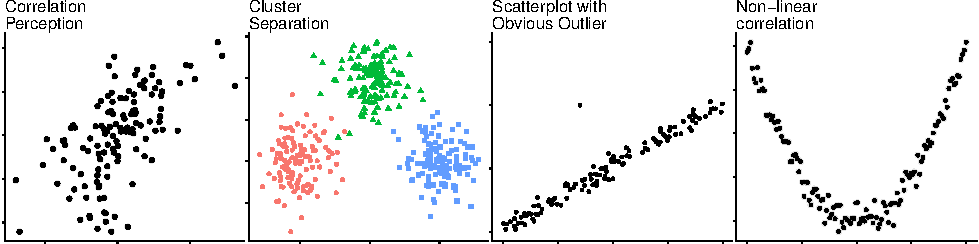
\includegraphics[width=1\textwidth,height=\textheight]{size_and_contrast_new_files/figure-pdf/fig-tasks-1.pdf}

}

\caption{\label{fig-tasks}Examples of scatterplots designed for
different scatterplot-associated tasks. Both colour and point shape have
been used to delineate different clusters in the cluster separation
plot.}

\end{figure}

\hypertarget{sec-related-work}{%
\section{Related Work}\label{sec-related-work}}

\hypertarget{sec-testing-corr-percept}{%
\subsection{Testing Correlation
Perception}\label{sec-testing-corr-percept}}

The testing of linear correlation perception in scatterplots has a long
and rich history, and has explored a wide variety of plot types, tasks,
and modelling methods. Work has had participants make discriminative
judgements between scatterplots with different correlations
\citep{pollack_1960, doherty_2007}, finding that performance on such a
task became better as the objective \emph{r} value increased. This
performance on a discriminative judgement task can also be modelled by
deep neural networks \citep{yang_2023}. Extensive work throughout the
1970's to 1990's focused primarily on having participants produce a
numerical estimate of correlation, finding evidence for a systematic
underestimation for positive \emph{r} values besides 0 and 1. This
underestimation was especially pronounced for 0.2 \textless{} \emph{r}
\textless{} 0.6
\citep{strahan_1978, bobko_1979, cleveland_1982, lane_1985, lauer_1989, collyer_1990, meyer_1992}
and is demonstrated using an equation relating objective to subjective
correlation \citep{rensink_2017} in
Figure~\ref{fig-underestimation-curve}. More recent work has attempted
to model participants' correlation estimation performance by using a
combination of bisection task, in which participants were asked to
adjust a plot until its correlation was halfway between two reference
plots, and a staircase task designed to produce Just Noticeable
Differences between scatterplots such that they are discriminable 75\%
of the time \citep{rensink_2010}. This work has also been extended to
incorporate Bayesian data analysis \citep{kay_2015}. The current
experiment takes similar techniques from previous work
\citep{strain_2023, strain_2023b} and combines them to further push the
envelope of how systematically adjusting visual features in scatterplots
can radically alter people's perceptions of correlation. For this reason
we use the same direct estimation paradigm to collect responses. This
paradigm allows for a large number of judgements to be collected, and is
simple enough that participants need little to no training.

\hypertarget{sec-drivers}{%
\subsection{Drivers of Correlation Perception}\label{sec-drivers}}

Evidence points towards correlation perception being driven by the shape
of the underlying probability distribution represented by scatterplot
points, however it should be noted that this is very much still an open
question, and it may be the case that there are different contributory
perceptual mechanisms operating at different levels based on
task-specific differences such as viewing time and levels of
graph-training. Increasing the \emph{x} and \emph{y} scales on a
scatterplot such that the size of the point cloud decreases
\citep{cleveland_1982} is associated with an increase in a viewer's
judgements of bivariate association, despite the objective \emph{r}
value remaining the same. It was suggested in this case that viewers may
have been using the area of the point cloud to judge association. Later
work found that the relationship between objective and perceived
\emph{r} values could be described by a function that included the mean
of the geometric distances between the points and the regression line
\citep{meyer_1997}. Investigations of the idea that people use visual
features to judge correlation provide evidence that, among others
features, the standard deviation of all perpendicular distances from
scatterplot points to the regression line was predictive of performance
on a correlation estimation task \citep{yang_2019}. Equations for both
discrimination and magnitude estimation of \emph{r} in scatterplots
include a quantity that is small when \emph{r} = 1 and increases as
\emph{r} approaches 0 \citep{rensink_2017}. This quantity is indifferent
to the type of visualization used, and is functionally similar to that
found in work mentioned above
\citep{cleveland_1982, meyer_1997, yang_2019}. Regarding scatterplots,
this quantity represents the average distance between data points and
the regression line, and can be thought of as representing the width of
the underlying distribution. Findings from deep neural networks also
support the idea that viewers are using an aspect of scatterplot shape
to judge correlation, or some measure of what has been termed \emph{dot
entropy} \citep{yang_2023}, again considered a candidate visual proxy
for correlation judgements \citep{rensink_2017, rensink_2022}.

Recent work investigating the use of decay functions that change point
size or contrast in scatterplots as a function of residual distance
provide further evidence for both point density and salience/perceptual
weighting being drivers of correlation perception. The use of an
inverted contrast decay function \citep{strain_2023}, such that point
contrast decreased as a point approached the regression line, resulted
in significantly lower and less accurate correlation estimates compared
to data-identical plots with the same overall shape, implying that the
center of the scatterplot not being \textbf{filled} biased viewers'
perceptions down. When point contrast or size are reduced as a function
of distance from the regression line \citep{strain_2023, strain_2023b},
viewers rate correlation as significantly higher and are significantly
more accurate, which supports a low-level data salience account. It is
more difficult to comment on higher level perceptual mechanisms, and in
any case this is not the intended contribution of the present work; we
aim to test the impact of systematically altering visual features on
correlation perception, and to provide empirically-derived tools for
visualization designers to design better visualizations through the use
of a simple, reproducible framework.

\begin{figure}

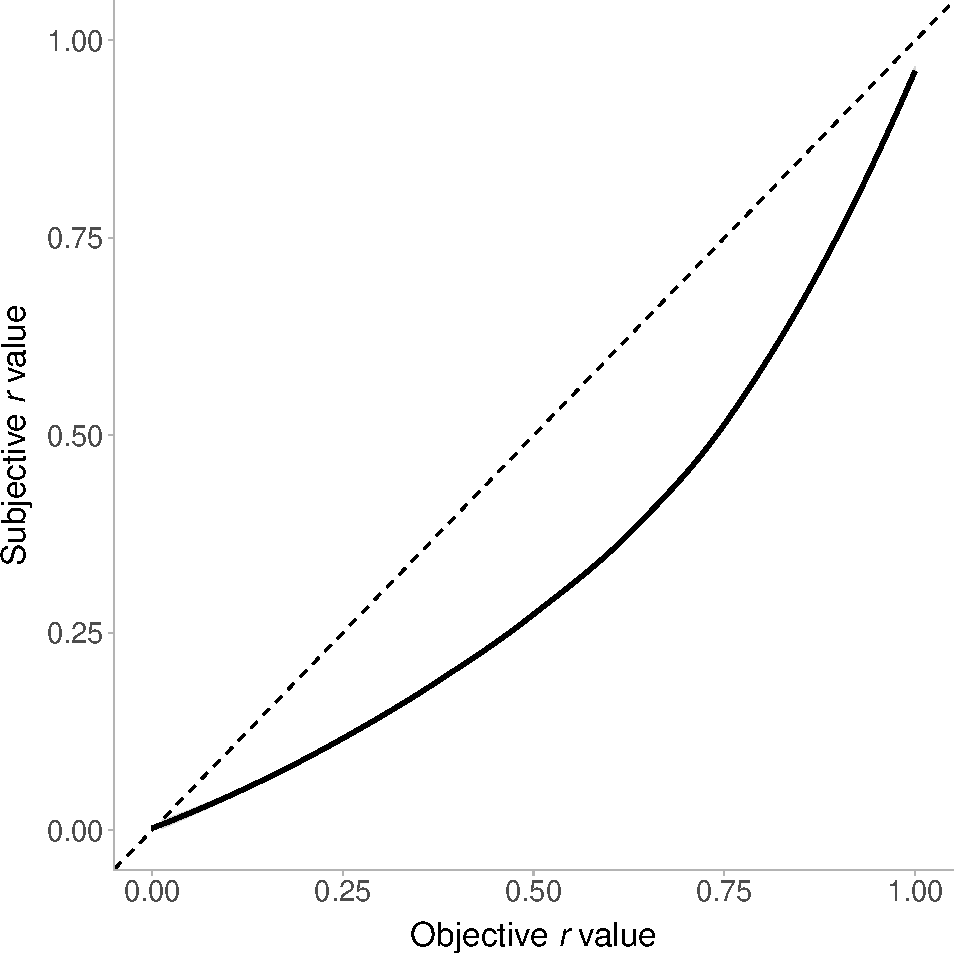
\includegraphics[width=0.5\textwidth,height=\textheight]{size_and_contrast_new_files/figure-pdf/fig-underestimation-curve-1.pdf} \hfill{}

\caption{\label{fig-underestimation-curve}Using a function relating
objective to perceived \emph{r} value \citep{rensink_2017} provides a
visualization of the nature of correlation underestmiation reported in
previous work. An identity line has been included to illustrate where
viewers are most and least accurate.}

\end{figure}

\hypertarget{sec-transparency-and-contrast}{%
\subsection{Transparency and
Contrast}\label{sec-transparency-and-contrast}}

Changing the contrast of scatterplot points is standard practice to deal
with issues of overplotting or clutter
\citep{matejka_2015, bertini_2004}; scatterplots with very large numbers
of points, especially with high degrees of overlap, suffer from low
individual-point visibility caused by high point density. Lowering the
contrast of all points addresses this, and makes data trends and
distributions easier to see and interpret (see
Figure~\ref{fig-overplotting-examples}).

\begin{figure}

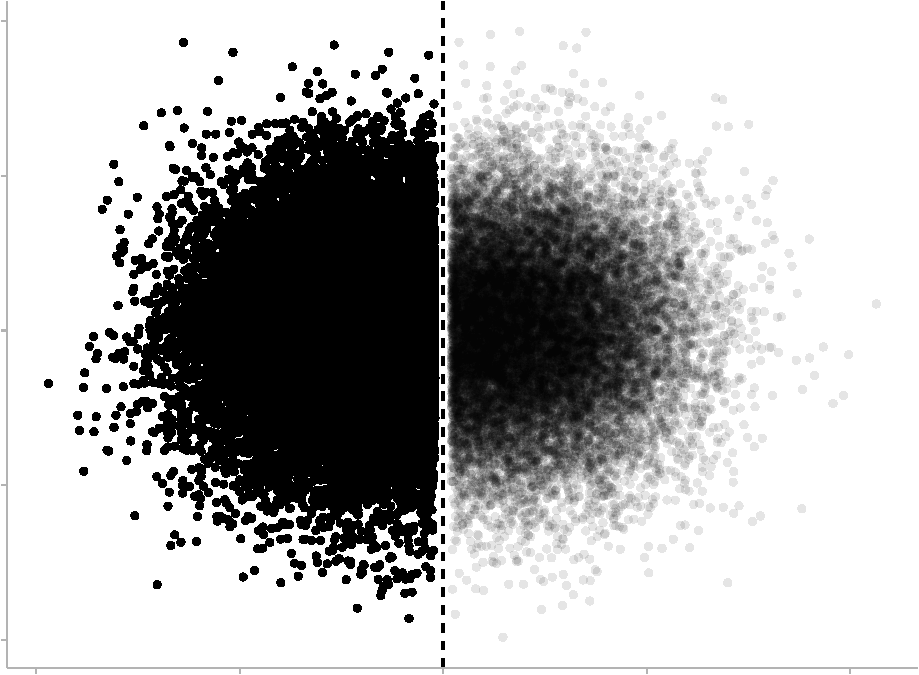
\includegraphics[width=0.5\textwidth,height=\textheight]{size_and_contrast_new_files/figure-pdf/fig-overplotting-examples-1.pdf} \hfill{}

\caption{\label{fig-overplotting-examples}Adjusting point contrast to
address overplotting. Contrast between the points and the background is
full (alpha = 1, L) or low (alpha = .1, R). The dataset used has 40,000
points.}

\end{figure}

\begin{figure}

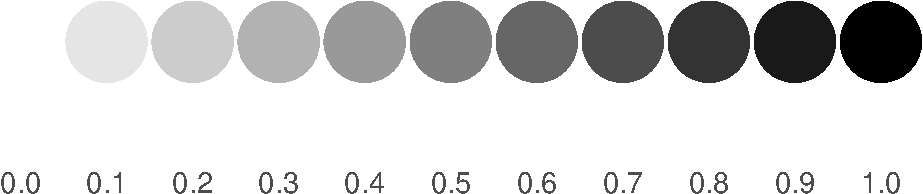
\includegraphics[width=0.5\textwidth,height=\textheight]{size_and_contrast_new_files/figure-pdf/fig-alpha-examples-1.pdf} \hfill{}

\caption{\label{fig-alpha-examples}Demonstrating the effects of
different alpha values on point contrast.}

\end{figure}

In the present study we use the \textbf{ggplot2} package
\citep{hadley_gg2016} to create our stimuli. This package uses an alpha
parameter, or the level of linear interpolation \citep{stone_2008}
between foreground and background pixel values, to set the contrast of
points. As demonstrated in Figure~\ref{fig-alpha-examples}, an alpha
value of 0 or 1 results in no interpolation and renders either the
background or foreground pixel values respectively. Psychophysical
definitions of perceived contrast are often based on what is being
presented (i.e gratings) or are modelled to take into account phenomena
of human vision (i.e visibility limits) \citep{zuffi_2007}. Our
crowdsourced methodology gives us no control the exact luminances of our
stimuli, only over the \emph{relative} differences in luminance between
scatterplot points and backgrounds. For this reason we do not report
absolute luminance nor make any attempt to adopt a formal definition of
contrast; instead we simply report the alpha value used. Given that our
work aims to improve correlation perception without removing data from
the scatterplot, we also incorporate point visibility testing (see
Section~\ref{sec-VT}). Informal point visibility piloting suggested that
our smallest, lowest contrast points had very low visibility. We
therefore implemented an alpha = 0.2 floor for these points, which we
felt conferred a sufficient level of point visibility.

Previous work has found that lowering the contrast of \emph{all}
scatterplot points relative to the background can increase the level of
underestimation error relative to full contrast, and that lowering point
contrast \emph{as a function of distance from the regression line} is
able to bias correlation estimates upwards to partially correct for the
underestimation bias \citep{strain_2023}. Evidence suggests point
salience/perceptual weighting and spatial uncertainty as drivers for
this effect. Lower stimulus contrast is associated with lower salience
\citep{healey_2011}, can bias judgements of mean point position
\citep{hong_2021} and increase error in positional judgements
\citep{wehrhahn_1990}, and can result in greater uncertainty in speed
perception \citep{champion_2017}. Due to effects of both
salience/perceptual weighting and spatial uncertainty operating in the
same direction, previous work \citep{strain_2023} has been unable to
determine the extent to which each is responsible for the observed
reduction in correlation estimation error.

\hypertarget{sec-point-size}{%
\subsection{Point Size}\label{sec-point-size}}

For discriminability reasons, scatterplots visualizing large datasets
tend also to have smaller points. Bubble charts are a subclass of
scatterplot which uses point size to describe a third variable, but what
little experimental work there is on the impact of point size on
correlation perception is inconclusive. Some work has found bias and
variability in correlation perception to be invariant to changes in
point size \citep{rensink_2012, rensink_2014}, while elsewhere a strong
effect of changing point size as a function of distance from the
regression line has been reported \citep{strain_2023b}. Evidence points
towards a salience-dominant mechanism in the latter case, albeit with a
small effect of spatial uncertainty. There is evidence that stimulus
size is associated with lower levels of spatial certainty
\citep{alais_2004} but higher levels of salience \citep{healey_2011},
and so the opposing directionality of predicted effects of
salience/perceptual weighting and spatial uncertainty on correlation
estimation has allowed researchers to provide evidence for the
mechanistic dominance of salience when point size is used.

\hypertarget{hypotheses}{%
\subsection{Hypotheses}\label{hypotheses}}

Based on previously established effects of adjusting point size and
point contrast using identical decay functions in isolation, we
presently make the following hypotheses about the combination of these
functions. We hypothesize that; (H1) an increased reduction in
correlation estimation error will be observed when standard orientation
decay functions are used; (H2) the use of congruent inverted orientation
decay functions will produce the least accurate estimates of
correlation; and (H3) that owing to the greater strength of the size
channel observed in previous work \citep{strain_2023b}, there will be a
significant difference in correlation estimates between the two
incongruent orientation conditions.

\hypertarget{sec-methods}{%
\section{Methodology}\label{sec-methods}}

\hypertarget{sec-crowdsourcing}{%
\subsection{Crowdsourcing}\label{sec-crowdsourcing}}

Much prior work into correlation perception in scatterplots has taken
place in-person, most often with graduate students with experience in
statistics. While this work is valuable, especially to perception
audiences, it can struggle to provide data that is resilient to
different lay viewers and viewing contexts. In addition, the ease and
low-cost afforded to us by online, crowdsourced experimental work is
unmatched. Given our intended HCI and design audience, we therefore
choose to crowdsource all participants. We acknowledge however, that the
technique has been affected by low quality data and skewed demographics
in the past \citep{chmielewski_2020, charalambides_2021, peer_2021}. In
light of these issues we follow published guidelines \citep{peer_2021}
to ensure the collection of high quality data. Namely, we use the
Prolific.co platform \citep{prolific} with stringent pre-screen
restrictions; participants were required to have completed at least 100
studies using Prolific, and were required to have a prolific score of
100, representing a 99\% approval rate. This is more strict than the
95\% suggested in previous work \citep{peer_2021}, but has served the
authors well in prior studies.

\hypertarget{sec-open-research}{%
\subsection{Open Research}\label{sec-open-research}}

This study was conducted according to the principles of open and
reproducible research. All data and analysis code are available at
(repository link removed for anon). This repository contains
instructions for building a docker image to fully reproduce the
computational environment used. This allows for full replications of
stimuli, analysis, and the paper itself. Ethical approval was granted by
(removed for anon). Hypotheses and analysis plans were pre-registered
with the OSF (links removed for anon) and there were no deviations from
them.

\hypertarget{sec-scatter-gen}{%
\subsection{Stimuli}\label{sec-scatter-gen}}

The data used to generate the scatterplots were identical to that used
in previous work \citep{strain_2023, strain_2023b}. 45 scatterplot
datasets were generated corresponding to 45 \emph{r} values uniformly
distributed between 0.2 and 0.99, as there is evidence that very little
correlation is perceived below \emph{r} = 0.2
\citep{strahan_1978, bobko_1979, cleveland_1982}. Using so many values
for \emph{r} allows us to paint a broader picture of people's
perceptions than work using fewer values. Scatterplot points were
generated based on bivariate normal distributions with standard
deviations of 1 in each direction. Each scatterplot had a 1:1 aspect
ratio, was generated as a 1000*1000 pixel .png image, and was scaled up
or down according to a participant's monitor such that they always
occupied the same proportion of the screen. We used equation 1 to map
residuals to size and contrast values. When adjusting point size, we
further transform values using a scaling factor of 4 and a constant of
0.2 t ensure that the minimum point size in the present study is
consistent with that of previous work \citep{strain_2023, strain_2023b}.

\begin{equation}
  point_{size/contrast} = 1 - b^{residual}
\end{equation}

0.25 was chosen as the value of \emph{b}. This is both due to its
previous usage in studies that the present work builds upon, and its
production of a curve approximating the inverse around the identity line
of the underestimation curve reported in previous work
\citep{rensink_2017, strain_2023, strain_2023b}. We acknowledge that
there may be other, more suitable values of \emph{b}, however extensive
testing of these is outside the scope of the present work. We used 2x2
combinations of this equation applied to point size and contrast in
standard and inverted orientation forms. Examples of the stimuli used
can be seen in Figure~\ref{fig-examples}.

\begin{figure}

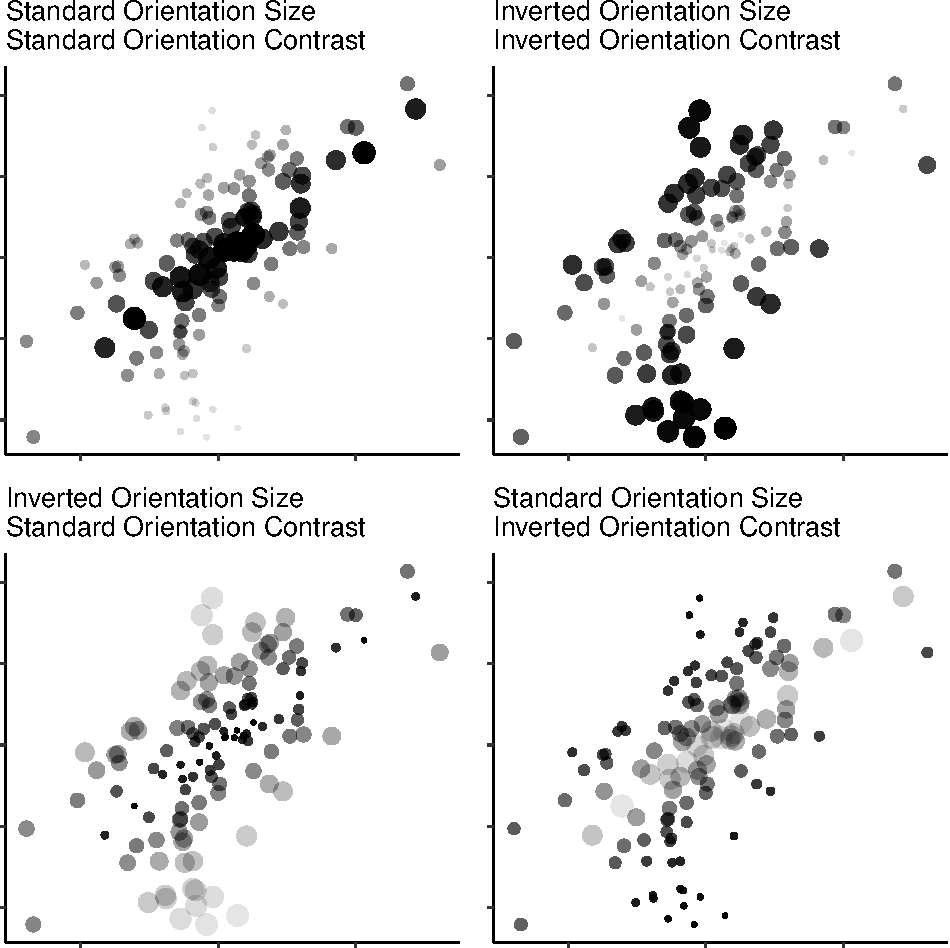
\includegraphics[width=0.5\textwidth,height=\textheight]{size_and_contrast_new_files/figure-pdf/fig-examples-1.pdf} \hfill{}

\caption{\label{fig-examples}Examples of the experimental stimuli used.}

\end{figure}

\hypertarget{sec-gen-modelling}{%
\subsection{Modelling}\label{sec-gen-modelling}}

We use linear mixed effects models to model the relationships between
the combination of size and contrast decay conditions and participants'
errors in correlation estimates. Models such as these allow us to
compare differences in our IV across the full range of participant
responses, as opposed to relying purely on aggregate data, as in ANOVA.
These models also afford us the ability to include random effects for
participants and items. As per our pre-registrations we preferred
maximal models, including random intercepts and slopes for participants
and items. The structures of these models was identified using the
\textbf{buildmer} package in R (version xx, \citep{voeten_buildmer}).
This package takes a maximal random effects structure and then
identifies the most complex model that converges, dropping terms that
fail to explain a significant amount of variance.

\hypertarget{sec-VT}{%
\subsection{Point Visibility Testing}\label{sec-VT}}

Discussions about the size and contrast of particular scatterplot points
are inherently difficult in the context of online, crowdsourced
experiments; controlling the devices participants use to participate in
these kind of experiments, beyond insisting on laptop or desktop
computers, is impossible. While this may result in a lack of consistency
in scatterplot point sizes, luminances, or contrast ratios between
participants, it also provides results that are more resilient to
different viewing contexts than traditional lab-based experimental work.
In addition to measures implemented to ensure high quality participant
data (see Section~\ref{sec-crowdsourcing}), it is also key that we do
not inadvertently remove data from scatterplots by including points
whose size or contrast renders them invisible. We therefore included
point visibility testing to ensure this. Participants viewed six
scatterplots that were made up of a certain number of points. These
points were of the same size and contrast as the smallest and lowest
contrast points used in the experimental items. Participants were asked
to enter in a textbox how many points were present. Participants scored
an average of 74.89\% (\(SD\) = 32.25). Despite our use of the contrast
floor detailed in Section~\ref{sec-transparency-and-contrast}, it is
clear that some of our small, low contrast points were not reliably
visible, most likely due to low contrast between the point and
background, as previous work \citep{strain_2023b} found point visibility
largely invariant to size. We suggest this is due to differences in
monitors between participants. In reality this contrast floor would need
to be calibrated on a per-monitor basis. Figure~\ref{fig-VT-hist} shows
distributions of participants' performances on the visibility tests. We
also include performance on the point visibility test as a fixed effect
in Section~\ref{sec-add-analyses}.

\begin{figure}

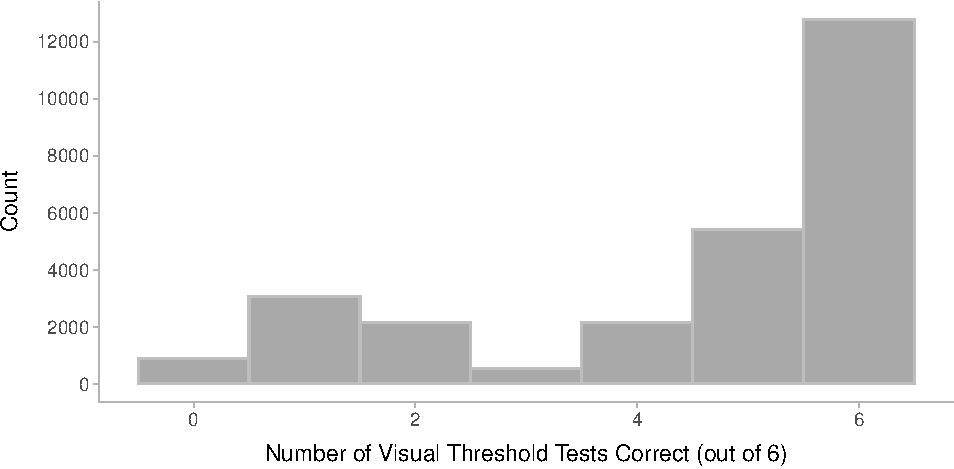
\includegraphics[width=0.5\textwidth,height=\textheight]{size_and_contrast_new_files/figure-pdf/fig-VT-hist-1.pdf} \hfill{}

\caption{\label{fig-VT-hist}Histogram of point visibility testing
performance.}

\end{figure}

\hypertarget{sec-dot-pitch}{%
\subsection{Dot Pitch}\label{sec-dot-pitch}}

We employed a method for obtaining the dot pitch of participants'
monitors \citep{screenscale}. Combining this with monitor resolution
information allows us to calculate the physical on-screen size of
scatterplot points. Participants were asked to hold a standard size
credit/ debit/ID card (ISO/IEC 7810 ID-1) up to their screen and resize
an on-screen card until the two matched. We assumed a widescreen 16:9
aspect ratio and calculated dot pitch based on these measurements. Mean
dot pitch was 0.34 (\(SD\) = 0.05). We include analyses with dot pitch
as a fixed effect in Section~\ref{sec-add-analyses}.

\hypertarget{sec-gen-procedure}{%
\subsection{Procedure}\label{sec-gen-procedure}}

Both experiments were built using PsychoPy \citep{pierce_2019} and
hosted on Pavlovia.org. Participants were only permitted to complete the
experiment on a desktop or laptop computer. Each participant was first
shown the participant information sheet and provided consent through key
presses in response to consent statements. They were asked to provide
their age in a free text box, followed by their gender identity.
Participants completed the 5-item Subjective Graph Literacy test
\citep{garcia_2016}, followed by the visual threshold task described in
Section~\ref{sec-VT} and the screen scale task described in
Section~\ref{sec-dot-pitch}. Participants were given instructions, and
were then shown examples of scatterplots with correlations of \emph{r} =
0.2, 0.5, 0.8, and 0.95, as piloting of a previous experiment indicated
some of the lay population may be unfamiliar with the visual character
of scatterplots. Section~\ref{sec-results} contains further discussion
of the potential training effects of this. Two practice trials were
given before the experiment began. Participants worked through a
randomly presented series of 180 experimental trials and were asked to
use a slider to estimate correlation to 2 decimal places. Visual masks
preceded each scatterplot. Interspersed were 6 attention check trials
which explicitly asked participants to ignore the scatterplot and set
the slider to 0 or 1.

\hypertarget{sec-participants}{%
\subsection{Participants}\label{sec-participants}}

150 participants were recruited using the Prolific.co platform. Normal
to corrected-to-normal vision and English fluency were required for
participation. In addition, participants who had completed any of our
previous studies into correlation estimation in scatterplots (references
removed for anon) were prevented from participating. Data were collected
from 158 participants. 8 failed more than 2 out of 6 attention check
questions, and, as per pre-registration stipulations, were rejected from
the study. Data from the remaining 150 participants were included in the
full analysis (50.7\% male, 48.7\% female, and 0.7\% non-binary).
Participants mean age was 30.6 (\emph{SD} = 8.6). Participants' mean
graph literacy score was 22.5 (\emph{SD} = 3.5). The average time taken
to complete the experiment was 37 minutes (\emph{SD} = 12.3).

\hypertarget{sec-design}{%
\subsection{Design}\label{sec-design}}

We used a fully repeated-measures 2*2 factorial design. Each participant
saw each combination of size and contrast decay condition plots for a
total of 180 experimental items. Participants viewed these experimental
items, along with 6 attention check items, in a fully randomized order.
All experimental code, materials, and instructions are hosted at (link
removed for anon).

\hypertarget{sec-results}{%
\section{Results}\label{sec-results}}

Our first two hypotheses were fully supported in this experiment. The
combination of standard orientation size and contrast decay functions
produced the most accurate estimates of correlation, although this also
resulted in a large correlation overestimation for many values of
\emph{r} (see Figure~\ref{fig-diff-error-bars-plot}). Our second
hypothesis was also supported; the combination of inverted size and
inverted contrast decay conditions produced the least accurate estimates
of correlation. We found no support for our third hypothesis; there was
no significant difference in correlation estimates for standard
orientation size/inverted orientation contrast decay plots and inverted
orientation size/standard orientation contrast decay plots (Z = -2.26,
\emph{p} = .11), however we did find a significant interaction effect
that provides evidence that the combination of size and contrast decay
functions is not additive in nature.

\hypertarget{tbl-sig}{}
\begin{table}
\caption{\label{tbl-sig}Significances of fixed effects and the interaction between them.
Semi-partial R\textsuperscript{2} for each fixed effect and the
interaction term is also displayed. }\tabularnewline

\centering
\begin{tabular}{lrrrrll}
\toprule
  & Estimate & Standard Error & df & t-value & \textit{p} & R\textsuperscript{2}\\
\midrule
(Intercept) & 0.08 & 0.013 & 103.32 & 6.27 & <0.001 & \\
Size Decay & -0.14 & 0.005 & 148.39 & -25.77 & <0.001 & 0.104\\
Contrast Decay & 0.12 & 0.002 & 26327.21 & 63.71 & <0.001 & 0.087\\
Size Decay x Contrast Decay & 0.15 & 0.004 & 26327.13 & 38.47 & <0.001 & 0.034\\
\bottomrule
\end{tabular}
\end{table}

All analyses were conducted using R (version 4.3.1). Deviation coding
was used for each of the experimental factors. We used the
\textbf{buildmer} and \textbf{lme4} packages to build a linear mixed
effects model where the difference between objective and rated r value
was predicted by the size and contrast decay conditions used. A
likelihood ratio test revealed that the model including point size and
contrast decay conditions as fixed effects explained significantly more
variance than the null (\(\chi^2\)(3) = 5,286.81, \emph{p} \textless{}
.001). There were significant fixed effects of size decay and contrast
decay conditions, as well as a significant interaction between the two.
The experimental model has random intercepts for items and participants,
and a random slope for the size decay factor with regards to
participants. Due both to our use of a linear mixed model with an
interaction term, and our lack of comparative baseline condition (i.e no
size or contrast function used), we do not report a measure of effect
size. Instead we report the amounts of variance explained by each fixed
effect term and the interaction term as semi-partial
R\textsuperscript{2} \citep{nakagawa_2013}. These values were calculated
using the \textbf{r2glmm} package \citep{r2glmm} can be see in
Table~\ref{tbl-sig} along with all model statistics.

\begin{figure}

{\centering 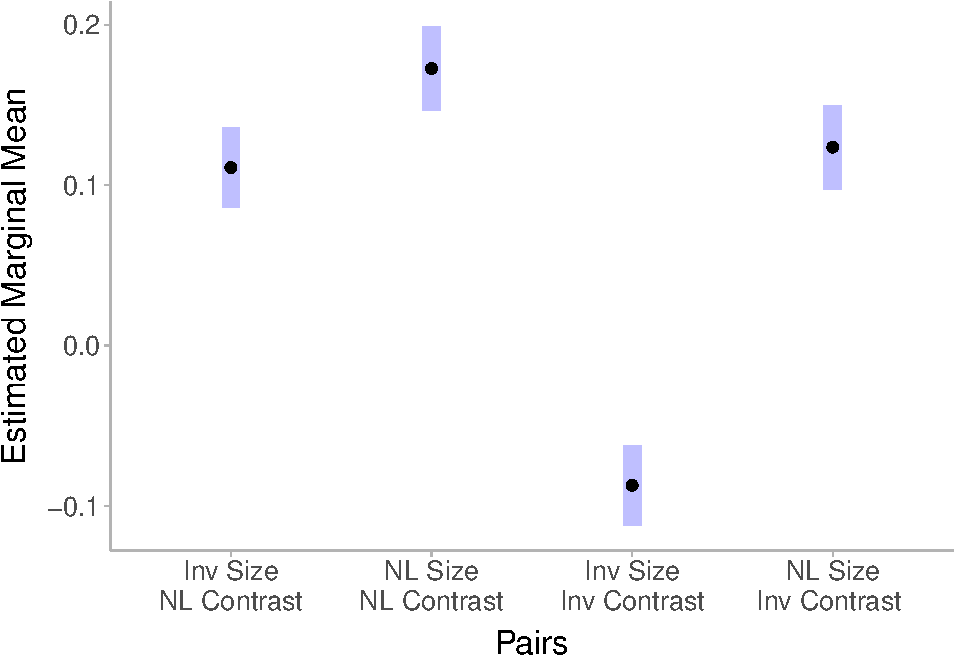
\includegraphics[width=1\textwidth,height=\textheight]{size_and_contrast_new_files/figure-pdf/fig-emm-plot-1.pdf}

}

\caption{\label{fig-emm-plot}Estimated marginal means for each
combination of size and contrast decay conditions, including asymptotic
lower and upper confidence limits calcualted by emmeans}

\end{figure}

\hypertarget{tbl-contrasts}{}
\begin{table}
\caption{\label{tbl-contrasts}Pairwise comparisons. SO = Standard Orientation, IO = Inverted
Orientation. The interaction is driven by the non-additive nature of
combining point size and contrast decay functions, and the only
nonsignificant contrast is found when incongruent decay functions are
tested. }\tabularnewline

\centering
\begin{tabular}{lrl}
\toprule
Contrast & Z.ratio & \textbackslash{}textit\{p\}\\
\midrule
SO Size x IO Contrast <-> IO Size x IO Contrast & -10.95 & <0.001\\
SO Size x IO Contrast <-> SO Size x SO Contrast & 72.29 & <0.001\\
SO Size x IO Contrast <-> IO Size x SO Contrast & -2.26 & 0.108\\
IO Size x IO Contrast <-> SO Size x SO Contrast & 46.13 & <0.001\\
IO Size x IO Contrast <-> IO Size x SO Contrast & 17.84 & <0.001\\
\addlinespace
SO Size x SO Contrast <-> IO Size x SO Contrast & -37.44 & <0.001\\
\bottomrule
\end{tabular}
\end{table}

\begin{figure}

{\centering 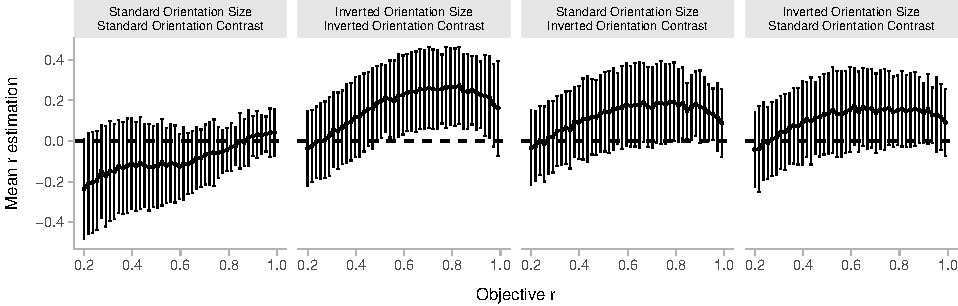
\includegraphics[width=1\textwidth,height=\textheight]{size_and_contrast_new_files/figure-pdf/fig-diff-error-bars-plot-1.pdf}

}

\caption{\label{fig-diff-error-bars-plot}Plots showing how participants'
correlation estimation errors change as a function of the \emph{r} value
for each combination of size and contrast decay factors.}

\end{figure}

\hypertarget{sec-add-analyses}{%
\subsection{Additional Analyses}\label{sec-add-analyses}}

We find no effects of graph literacy (\(\chi^2\)(1) = 3.50, \emph{p} =
.061) or performance on the visual threshold task (\(\chi^2\)(1) = 1.29,
\emph{p} = .257), or dot pitch (\(\chi^2\)(1) = 1.52, \emph{p} = .218)
on participants' errors in correlation estimation.

\hypertarget{sec-discussion}{%
\section{Discussion}\label{sec-discussion}}

Our findings here provide further confirmatory evidence of what has been
found previously with regards to the effects of point size and contrast
manipulations on correlation estimation in scatterplots. Namely, that
while both manipulations have a significant effect, the effect of
changing point sizes is stronger, and that while we can influence
correlation estimates in either direction, standard orientation
manipulations are more powerful than inverted ones
\citep{strain_2023, strain_2023b}. As one would expect, we also see an
effect of orientation congruency on the extent to which a manipulation
can bias correlation estimates.

The lack of support for our third hypothesis, that there would be a
difference in correlation estimates between incongruent conditions, was
surprising given the greater strength of the size channel relative to
contrast demonstrated in previous work
\citep{strain_2023, strain_2023b}. Despite the lack of support for this
hypothesis, we did find that the size decay channel explained more
variance (.104) in our model than contrast decay (.087) was able to. If
the combination of size and contrast decay functions was strictly
additive, we would expect a significant difference between incongruent
conditions owing to the greater power of the size channel. Their
non-additive nature, however, has resulted in each channel attenuating
the other.

\hypertarget{combining-manipulations}{%
\subsection{Combining Manipulations}\label{combining-manipulations}}

Figure~\ref{fig-diff-error-bars-plot} and Figure~\ref{fig-emm-plot} show
how, on average, the combination of standard orientation size and
contrast decay conditions has resulted in an overestimation of \emph{r}
for the majority of values. While this does not directly solve the
underestimation problem. It does demonstrate that with regards to using
point size and contrast to bias viewer's estimates of correlation in
scatterplots, there would appear to be few limitations. The issue here
is not one of ability to change people's perceptions, but of
\emph{tuning} the use of these visual factors to be able to change
people's perceptions in systematic ways. We explore what further work
would need to be done to do this in Section~\ref{sec-future-work}.

\hypertarget{contributions-of-size-and-contrast-decay}{%
\subsection{Contributions of Size and Contrast
Decay}\label{contributions-of-size-and-contrast-decay}}

Incorporating data from previous work \citep{strain_2023, strain_2023b}
that used similar decay functions and experimental paradigms allows us
to compare estimation curves for size decay and contrast decay in
isolation and in combination (Figure~\ref{fig-est-multi-exp}). We can
then derive new curves that describe the effect that each manipulation
and the combination of manipulations has on people's estimates of
correlation (Figure~\ref{fig-power-plot}). Throughout the course of this
section it should be noted that the analyses include data from several
separate experiments. We argue that their methodological similarities
render comparison appropriate, but we acknowledge the potential for
overstated conclusions.

\begin{figure}

{\centering 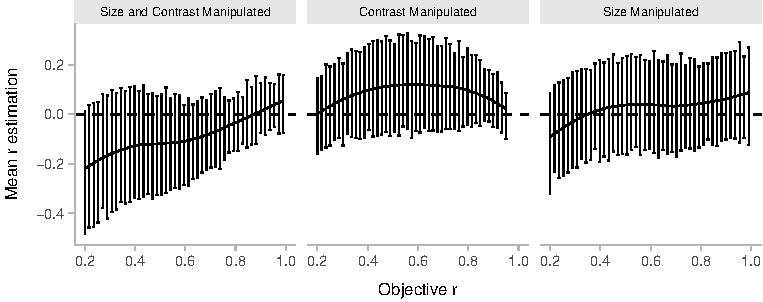
\includegraphics[width=1\textwidth,height=\textheight]{size_and_contrast_new_files/figure-pdf/fig-est-multi-exp-1.pdf}

}

\caption{\label{fig-est-multi-exp}From left to right, plotting \emph{r}
estimation error against the objective \emph{r} value for the standard
orientation condition in the present study, for standard orientation
size and contrast manipulations in previous work, and for normal
scatterplots averaged over identical conditions in previous work. Error
bars have been left off this plot to make interpretation more simple.}

\end{figure}

\begin{figure}

{\centering 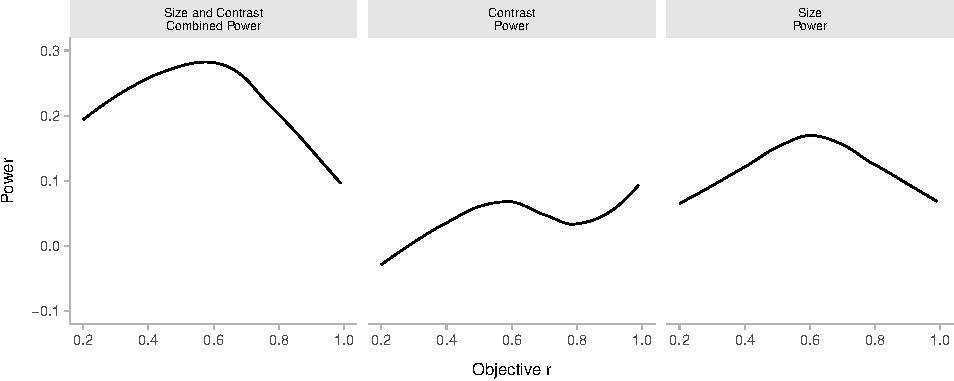
\includegraphics[width=1\textwidth,height=\textheight]{size_and_contrast_new_files/figure-pdf/fig-power-plot-1.pdf}

}

\caption{\label{fig-power-plot}additive\_raw\_pl = observed values for
present study. standard\_curve = no manipulation averaged across all
experiments}

\end{figure}

\hypertarget{sec-mechs}{%
\subsection{Mechanisms}\label{sec-mechs}}

\hypertarget{sec-further-tuning}{%
\subsection{Further Tuning}\label{sec-further-tuning}}

\hypertarget{sec-limitations}{%
\subsection{Limitations}\label{sec-limitations}}

\hypertarget{sec-future-work}{%
\subsection{Future Work}\label{sec-future-work}}

\bibliographystyle{ACM-Reference-Format}
\bibliography{size-contrast-new.bib}

%% begin pandoc before-bib
%% end pandoc before-bib
%% begin pandoc biblio
%% end pandoc biblio
%% begin pandoc include-after
%% end pandoc include-after
%% begin pandoc after-body
%% end pandoc after-body

\end{document}
\endinput
%%
%% End of file `sample-manuscript.tex'.
